% !TEX = root../thesis.tex

\chapter{Real Time Muon Reconstruction at the Compact Muon Solenoid}
\label{chap:kbmtf}

\section{Introduction} \label{sec:kbmtf_intro}
Section~\ref{sec:CMS_L1T} provides an overview of the L1 trigger and its importance to the CMS trigger system. This section will detail the design and performance of a Kalman Filter algorithm used in the L1 trigger to identify muon tracks in the barrel region ($|\eta|<0.83$) of the CMS detector. This algorithm, known as the Kalman Barrel Muon Track Finder (KBMTF), was fully implemented for 2018 data taking and received improvements for continued use in Run-3.

The L1 barrel muon trigger receives inputs from the TwinMux system, which creates trigger primitives by combining information from the DT and RPC detectors to determine the position, trajectory, and timing of hits from incident muons at each station~\cite{Triossi_2017}. These hits, referred to as "stubs", are fed to the L1 muon trigger electronics where they are used to reconstruct muon tracks. The previous track finding algorithm, known as the Phase-I Barrel Muon Track Finder (BMTF), used a maximum of two stubs to reconstruct muon trajectories and was designed under the assumption that muons originate only from the beam line. As a part of upgrading the L1 Trigger, the KBMTF algorithm was developed to utilize stubs from all four muon stations as well as reconstruct displaced muon tracks resulting from decays of exotic long lived particles.

\section{The Kalman Filter Algorithm} \label{sec:kalman_filter}
A Kalman Filter is a tracking algorithm that performs a recursive, iterative chi-square-like fit. Qualitatively, it propagates a system from its current state to the next and combines the predicted value with measurements to "update" the state of the system. This updated system is then iteratively propagated and updated with new measured values. This section focuses on a discrete linear Kalman Filter, which is applicable when a system can be described with a vector of variables whose evolution can be modeled with a linear transformation plus random uncertainties~\cite{FRUHWIRTH1987444}.

Abstractly, the state of a system at a given step $n-1$ can be described by a vector labeled $x_{n-1}$ with covariance matrix $P_{n-1}$. Let the matrix $F_n$ represent the linear transformation that propagates $x_{n-1}$ to the next state $x_{n}$, and the matrix $Q_{n}$ be the covariance matrix due to additional uncertainty. The predicted state of the system at step $n$ can be given by
\begin{equation}
	\label{eq:prop}
	x_{n}=F_{n}x_{n-1} \quad \textrm{and} \quad P_{n}=F_nP_{n-1}F_n^T+Q_n
\end{equation}
where $F_nP_{n-1}F_n^T$ represents the propagation of the initial covariance matrix.

Now define a set of measurements taken at state $n$ as $z_n$ with covariance matrix $R_n$. The measured variables are not restricted to the same set of variables defining $x_n$ as long as there exist a "change of basis" matrix $H$ that relates the sets. It should be noted that mathematically $H$ is not a strict change of basis matrix, as the measured values can have smaller dimensionality than the propagated ones. The predicted state and covariance matrix of the system written in the same variables as the measured quantities are defined as
\begin{equation}
	\label{eq:changeOfBasis}
	\mu_n=Hx_n \quad \textrm{and} \quad \Sigma_n=HP_nH^{T}
\end{equation}

Updating the system relies on a matrix known as the Kalman Gain, which acts as a weight based on $\Sigma_n$ and $R_n$ and determines if the updated system should skew more towards the measured or predicted values. The Kalman gain is defined as
\begin{equation}
	\label{eq:gain}
	K\coloneqq \Sigma_n\left(\Sigma_n+R_n\right)^{-1}
\end{equation}
which is then used to calculate the updated system as follows
\begin{equation}
	\label{eq:update1}
	\mu_n'=\mu_n+K\left(z_n-\mu_n\right) \quad \textrm{and} \quad \Sigma_n'=\Sigma_n-K\Sigma_n
\end{equation}

The term $z_n-\mu_n$ is frequently referred to as the residual of the prediction and measured value. A Kalman gain equal to the identity $I$ would set the updated coordinates to the measured values, while a Kalman gain of $0$ would effectively ignore the measured values. Finally, we substitute $x_n$ and $P_n$ into equation~\ref{eq:update1} using equation~\ref{eq:changeOfBasis} and simplify to give
\begin{equation}
	x_n'=x_n+K'(z_n-Hx_n) \quad \mathrm{and} \quad P_n'= P_n-K'HP_n
\end{equation}
where the Kalman Gain $K$ has been redefined to
\begin{equation} \label{eq:gain2}
	K'=P_nH^T(HP_nH^T+R_n)^{-1}
\end{equation}
The system $x_n'$ and $P_n'$ can now be propagated to step $n+1$ where the Kalman Algorithm can be iterated.

\section{The Kalman Barrel Muon Track Finder} \label{sec:kbmtf}
A rough outline KBMTF algorithm for track finding is as follows:
\begin{enumerate}
	\item A track seed is chosen from a stub in the muon station, from which a preliminary track is built. This seed cannot be chosen from the innermost muon station.
	\item The track is propagated inward to the next station and matched to the closest stub. If there is a matching stub, update the track with the stub information. Repeat until the track is at the innermost station. \label{kbmtf_step2}
	\item The track is propagated from the innermost station to the beam axis. The track properties at this point are stored as the "vertex unconstrained" measurement. These properties include the $p_T$, $\phi$, $\eta$, and $d_{xy}$, which is defined as the closest distance from the propagated track to the beam axis. \label{kbmtf_step3}
	\item The vertex propagated track is updated with the constraint that the track originated from the beam axis, and the track properties are stored as the "vertex constrained" measurement. \label{kbmtf_step4}
\end{enumerate}

Muon track finding begins at the outer stations in order to get both the vertex unconstrained measurement and the vertex constrained measurement with only one iteration of the KBMTF algorithm. Starting from the inner station and propagating outward would require an additional propagation back inward in order to get the vertex constrained measurement, which would cause the algorithmic latency to exceed timing restrictions. The outer stations are also the lowest occupancy, meaning stubs are less likely to be from background. Tracks are then overlap cleaned, which ensures that stubs are not shared among multiple tracks, and cut and selected based on various goodness of fit criteria. A diagram showing the KBMTF propagation and update procedure can be shown in figure~\ref{fig:kbmtf}.

\begin{figure} [htb!]
	\centering
	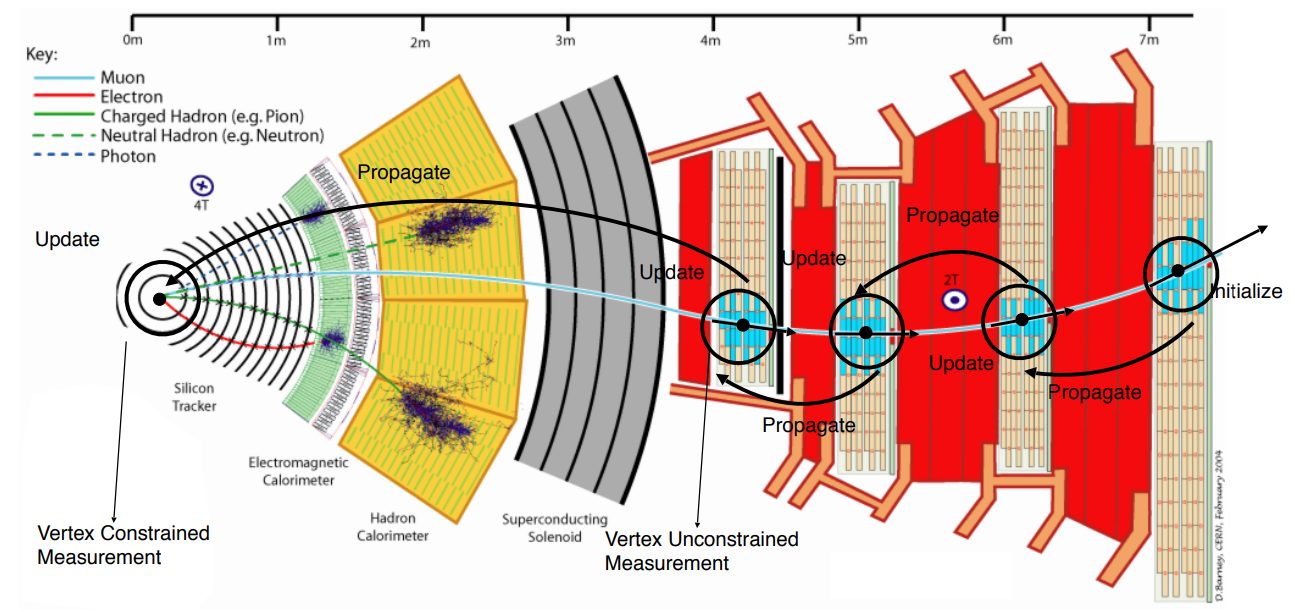
\includegraphics[width=0.85\linewidth]{figs/04_muons/kbmtf_diagram.png}
	\caption[The iterative process of propagation and updating a muon track through the KBMTF algorithm. The track properties at the innermost station are stored in order to trigger on muons not originating from the beam axis~\cite{CERN-LHCC-2020-004}]
	{The iterative process of propagation and updating a muon track through the KBMTF algorithm. The track properties at the innermost station are stored in order to trigger on muons not originating from the beam axis~\cite{CERN-LHCC-2020-004}.}
	\label{fig:kbmtf}
\end{figure}

\subsection{Muon Trajectory Propagation} \label{sec:muons_prop}
In order to implement a Kalman Filter, the propagation of muon tracks between stations must be expressed as a linear function of the track variables. From equation~\ref{eq:pt03br}, a charged particle will travel in a circular orbit in the $\hat{r}-\hat{\phi}$ plane. The high center of mass energy of the LHC results in highly energetic particles, whose trajectories have radii substantially larger than the size of the CMS detector. The large radius of curvature allows us to approximate these trajectories as parabolas. Assume a Cartesian coordinate system with the origin placed along a particle's trajectory that has radius R. This trajectory can then be approximated as
\begin{equation}
	\label{eq:parabola1}
	y(x)=\frac{x^2}{2R}+bx
\end{equation}
where $b$ is a coefficient depending on the orientation of the coordinate system. If the initial trajectory is defined as $\phi_{b,0}$, taking the derivative and evaluating at the origin yields
\begin{equation}
	\label{eq:phib}
	y'(0)=\tan(\phi_{b,0})=b
\end{equation}	
The curvature $k=q/p_{T}$, where the muon charge $q=\pm1$, is the preferred variable to work with when propagating the trajectory of a muon, as the propagation is linear in $k$. Substituting values from equations~\ref{eq:pt03br} and~\ref{eq:phib} into equation~\ref{eq:parabola1} yields
\begin{equation}
	\label{eq:parabola2}
	y(x)=akx^2+\tan(\phi_{b,0})x
\end{equation}
where $a=\frac{0.3B}{2}$. Muon hits, or "stubs", provide information on the position $\phi$ and bending angle $\phi_b$. Let the radius of two sequential muon stations be $r_1$ and $r_2$, with the outer radius given by $r_2$ and $\Delta r=r_2-r_1$. Assuming a muon has curvature $k$ at the outer station and ignoring energy loss, equation~\ref{eq:parabola2} can be used to propagate stubs from the outer station towards the inner station.
\begin{equation}
	y(-\Delta r) = \left(a\Delta r^2\right)k-\Delta r\tan(\phi_{b,0})
\end{equation}
\begin{equation}
	y'(-\Delta r)=-\left(2a\Delta r\right)k+\tan(\phi_{b,0})
\end{equation}
Converting these to the quantities to angles measured by the detector yields
\begin{equation}
	\label{eq:prop_phi}
	\tan(\Delta\phi)=\frac{y(-\Delta r)}{r_1}
\end{equation}
\begin{equation}
	\label{eq:prop_phib}
	\phi_b=\Delta\phi+\mathrm{tan}^{-1}\left[y'(-\Delta r)\right]
\end{equation}
The $\Delta\phi$ term is added to equation~\ref{eq:prop_phib} because the bending angle at each station is measured relative to an axis system oriented towards the center of the detector. Due to the large radius of curvature of the muon trajectories, the small angle approximation $\tan(x)\sim \tan^{-1}(x)\sim x$ can be applied, giving the equations
\begin{equation}
	\label{eq:prop_phi_approx}
	\Delta\phi=\frac{a\Delta r^2}{r_1}k-\frac{\Delta r}{r_1}\phi_{b,0}
\end{equation}
\begin{equation}
	\label{eq:prop_phib_approx}
	\phi_b=a\Delta r\left(\frac{\Delta r}{r_1}-2\right)k+\left(\frac{r_2}{r_1}\right)\phi_{b,0}
\end{equation}
A diagram showing this propagation can be seen in figure~\ref{fig:mu_trajectory}.

\begin{figure}[h!]
	\centering
	%Final image: origin at outer stub, oriented with x axis pointing towards vertex
	% !TEX = root../../thesis.tex
\begin{tikzpicture}
	% axis system
	\draw[thick,->] (-11, 0) -- (1, 0) node[anchor=west] {x};
	\draw[thick,->] (0, 0) -- (0, 4) node[anchor=south] {y};
	\coordinate[label = above left:$\mathrm{Vertex}$] (vertex) at (-9.5, 0);
	\coordinate[label = above right:$\mathrm{Origin}$] (origin) at (0, 0);
	\coordinate[] (r1) at (-5, 0);
	\node at (vertex)[circle,fill,inner sep=2pt]{};
	\node at (origin)[circle,fill,inner sep=2pt]{};
	\draw[<->] (-9.5, -.5) -- (-5, -.5);
	\draw[<->] (-9.5, -1.1) -- (0, -1.1);
	\coordinate[label = below:$r_1$] (r1) at (-7.25,-.5);
	\coordinate[label = below:$r_2$] (r2) at (-5,-1.1);
	\draw[dashed] (-5, 0) -- (-5, 4);
	
	% muon trajectory
	\def \X{2.6047227}; %circle x0
	\def \Y{14.772116}; %circle y0
	
	\def \sy{1.8427620};%stub at (-5, y)
	\draw [{Latex[length=3mm]}-, domain=270:230] plot ({\X+15*cos(\x)}, {\Y+15*sin(\x)});
	\draw ({\X+15*cos(230)}, {\Y+15*sin(230)}) node[font=\bfseries, anchor=east] {$\mu$};
	\draw (-2.25,.25) node[anchor=west] {$\phi_{b,0}$};
	\coordinate[] (stub1) at (-5, \sy);
	\draw [dashed, domain=0:6] plot ({-9.5+\x}, {0.40950267*\x});
	\draw [dashed] (-5, \sy) -- (-4, \sy);
	\draw (-8.5, .25) node[anchor=west] {$\Delta\phi$};
	\draw (-4, \sy) node[anchor=west, scale=1.0] {$\phi_b$};
	\draw (-4.5, \sy+.1) node[anchor=west, scale=0.7] {$\Delta\phi$};
\end{tikzpicture}
	\caption{Diagram showing a muon trajectory between two stations with the origin set at the outer station. The x-axis is oriented using the detector vertex and the outer station.}
	\label{fig:mu_trajectory}
\end{figure}

Equations~\ref{eq:prop_phi_approx} - \ref{eq:prop_phib_approx} show that the track propagation fits the criteria for a discrete linear Kalman Filter discussed in section~\ref{sec:kalman_filter}. The matrices for propagation can now be constructed as follows. The transfer matrix $F_n$ from equation~\ref{eq:prop} can be expressed as
\begin{equation}
	\label{eq:kmtfProp}
	x_{n}=\left(\begin{matrix}
		k\\
		\phi\\
		\phi_b
	\end{matrix}\right)_{n} = 
\left(\begin{matrix}
	1 & 0 & 0\\
	\alpha_n & 1 & -\frac{\Delta r}{r_n}\\
	\beta_n & 0 & \frac{r_{n-1}}{r_n}
\end{matrix}\right)
\left(\begin{matrix}
	k\\
	\phi\\
	\phi_b
\end{matrix}\right)_{n-1}=F_nx_{n-1}
\end{equation}
where the coefficients
\begin{equation}
	\label{eq:kmtf_coeff}
	\alpha_n=a\frac{\Delta r^2}{r_n} \quad \mathrm{and} \quad \beta_n=a\Delta r\left(\frac{\Delta r}{r_n}-2\right)
\end{equation}
with $r_{n-1}$ being the radius of the previous (outer) muon station and $r_n$ the radius of the sequential (inner) muon station.

While the radii of the muon stations are determined by detector geometry, the constants $\alpha_n$ and $\beta_n$ are measured using single muon monte-carlo samples where stubs are matched to the incident muons using generator level information. To determine $\alpha_n$, stubs in stations $n$ and $n-1$ are first associated if they resulted from the same incident muon. For matching stubs, the quantity $\Delta\phi+\frac{\Delta r}{r_1}\phi_{b,0}$ is plotted versus the muon $k$ in a 2-dimensional histogram. Slices along the y-axis are fit using a Gaussian distribution, and the mean value for each slice is used to calculate a linear fit as a function of $k$. $\beta_n$ is calculated similarly by plotting $\phi_b-\left(r_{n-1}/r_n\right)\phi_{b,0}$ vs $k$. This process can be seen in figure~\ref{fig:phi_prop}.

\begin{figure}[htb!]
	\centering
	\captionsetup{justification=centering}
	\begin{subfigure}[b]{0.45\textwidth}
		\centering
		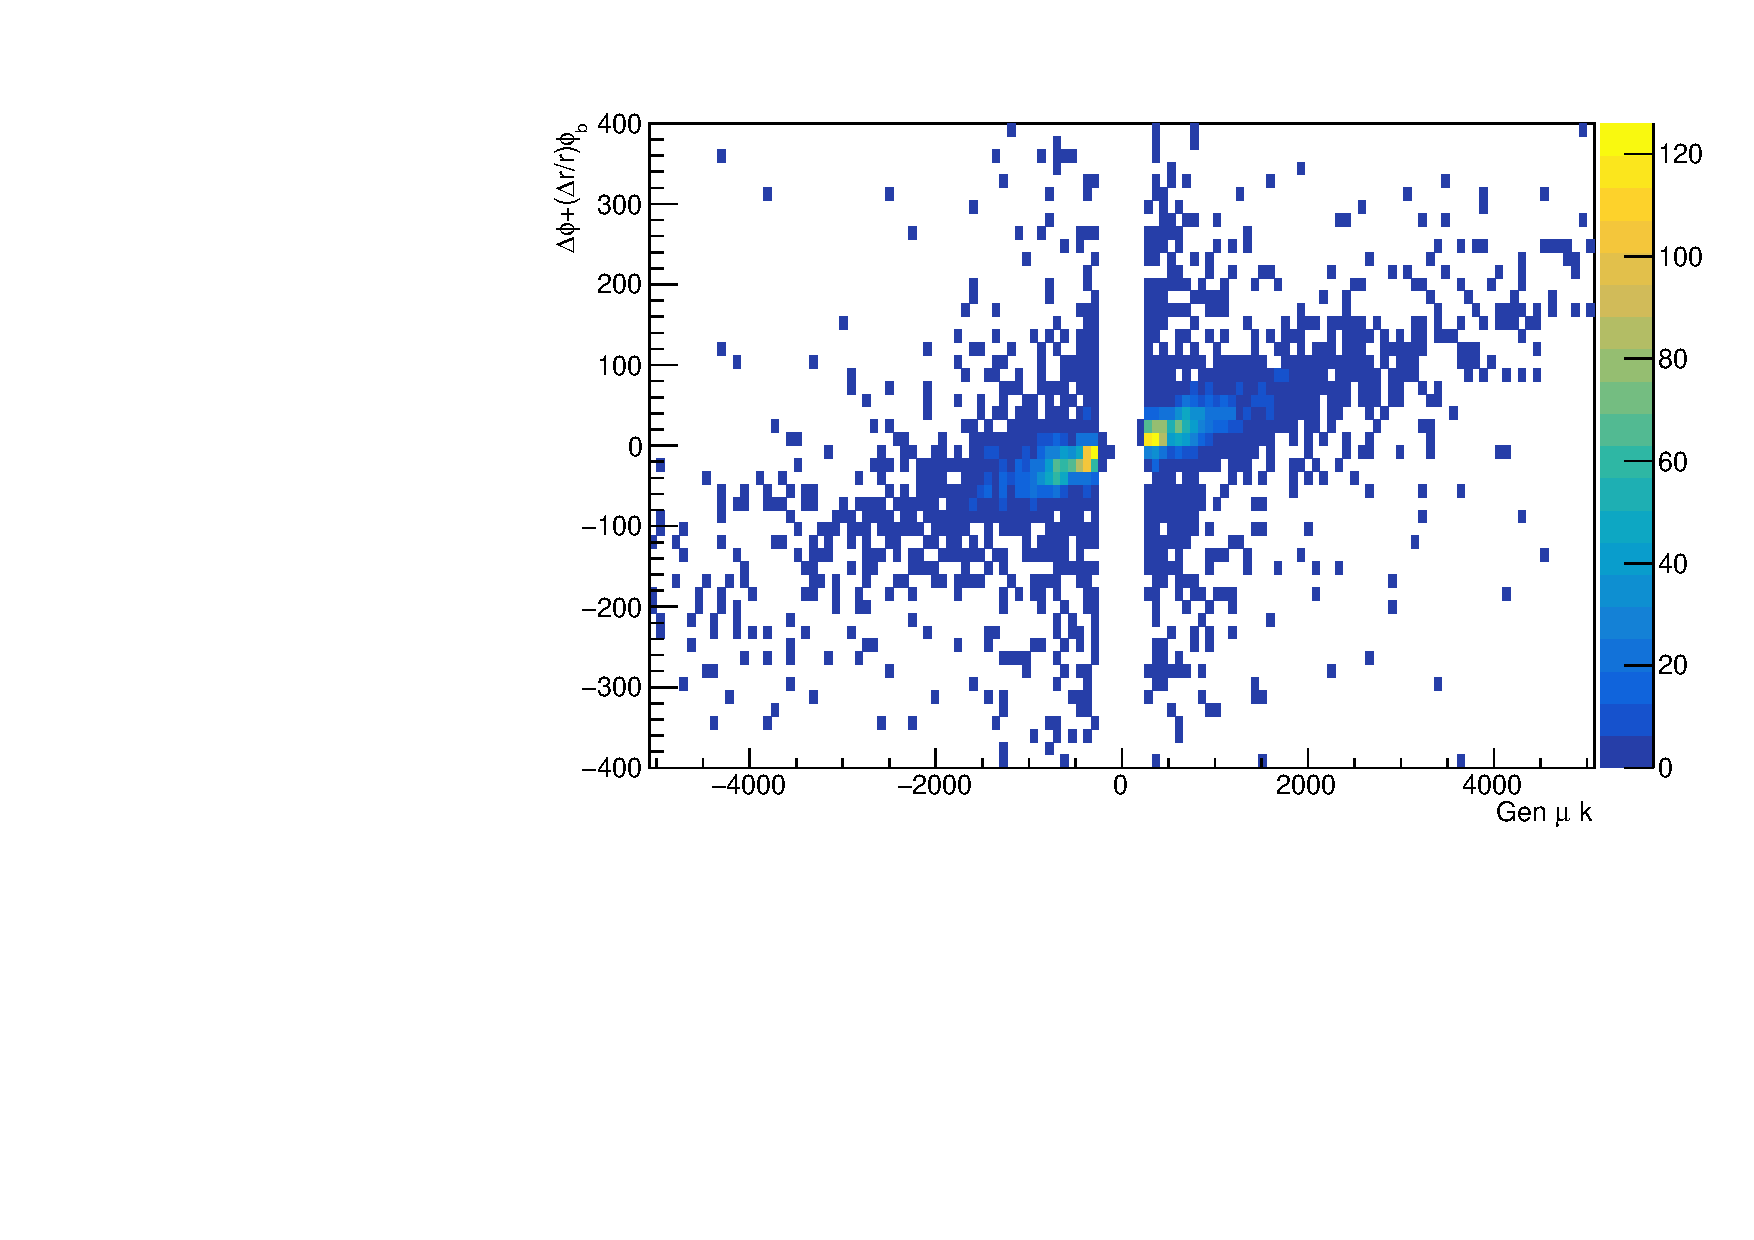
\includegraphics[width=\textwidth]{figs/04_muons/phiprop_2d.pdf}
		\caption{2-dimension histogram of $\Delta\phi+\frac{\Delta r}{r_1}\phi_{b,0}$ vs $k$.}
		\label{fig:2dprop}
	\end{subfigure}\hspace{0.05\textwidth}
	\begin{subfigure}[b]{0.45\textwidth}
		\centering
		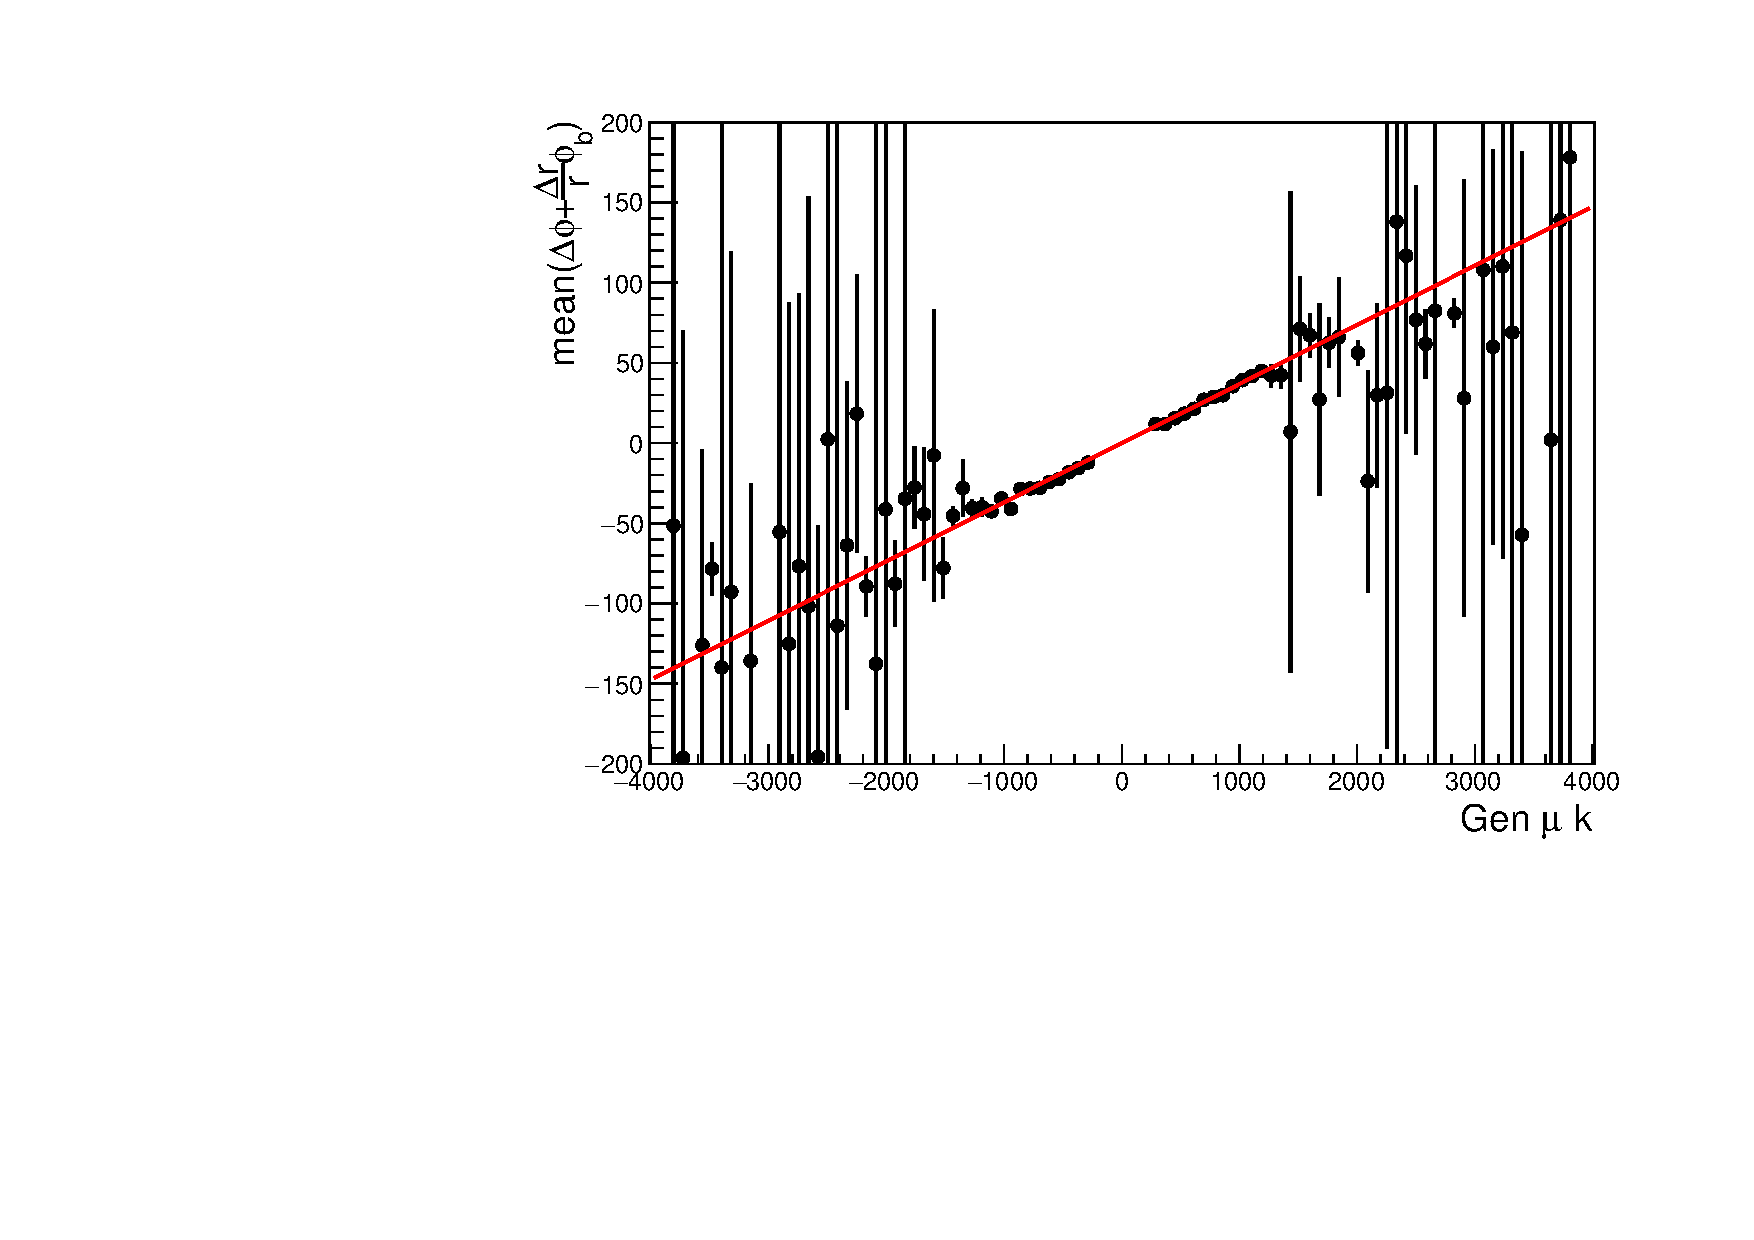
\includegraphics[width=\textwidth]{figs/04_muons/phiprop_mean.pdf}
		\caption{Mean of vertical slices fits used to calculate $\alpha$.}
		\label{fig:2dprop_mean}
	\end{subfigure}
	\caption[Calculation of phi propagation coefficients. Units are converted to their digitized form used in firmware calculations.]
	{Calculation of phi propagation coefficients. Units are converted to their digitized form used in firmware calculations.}
	\label{fig:phi_prop}
\end{figure}

\subsection{Covariant Matrices and the Kalman Gain} \label{sec:kbmtf_cov}
There are two sources of uncertainty that affect the covariance matrices. The first is multiple coulomb scattering, which occurs when muons scatter elastically with material in the detector. This can be thought of as a small deflection in momentum that alters the trajectory the muon. Lower momentum muons will be deflected at greater angles, so this uncertainty is proportional to $k$. Additionally, the probability for multiple scattering is proportional to the amount of material traversed by the muon, so this uncertainty must be calculated for each step in propagation. This is an uncertainty resulting from the propagation, and therefore plays the role of $Q_n$ from equation~\ref{eq:prop}. The second source is from the intrinsic detector resolution, which is a fixed value for each detector. However, the angular resolution is dependent on the radial distance from the center of the detector, so these must be calculated for each station as well. Since this is an uncertainty on the measurements, the resolution plays the role of $R_n$ in equation~\ref{eq:gain}. The total uncertainty resulting from both of these factors is given by
\begin{equation}
	\label{eq:prop_uncertainty}
	\sigma(k)=\sqrt{\sigma_{ms}^2k^2+\sigma_{res}^2}
\end{equation}

The coefficients can be calculated by using the Gaussian slice fits described when deriving $\alpha$ and $\beta$. For each propagation, the sigma of the Gaussian fits is plotted versus $k$ and fit to the form in equation~\ref{eq:prop_uncertainty}. This fitting process for $\phi$ propagation coefficients is shown in figure~\ref{fig:phi_uncertainty}, and is functionally the same for $\phi_b$.

\begin{figure}[htb!]
	\centering
	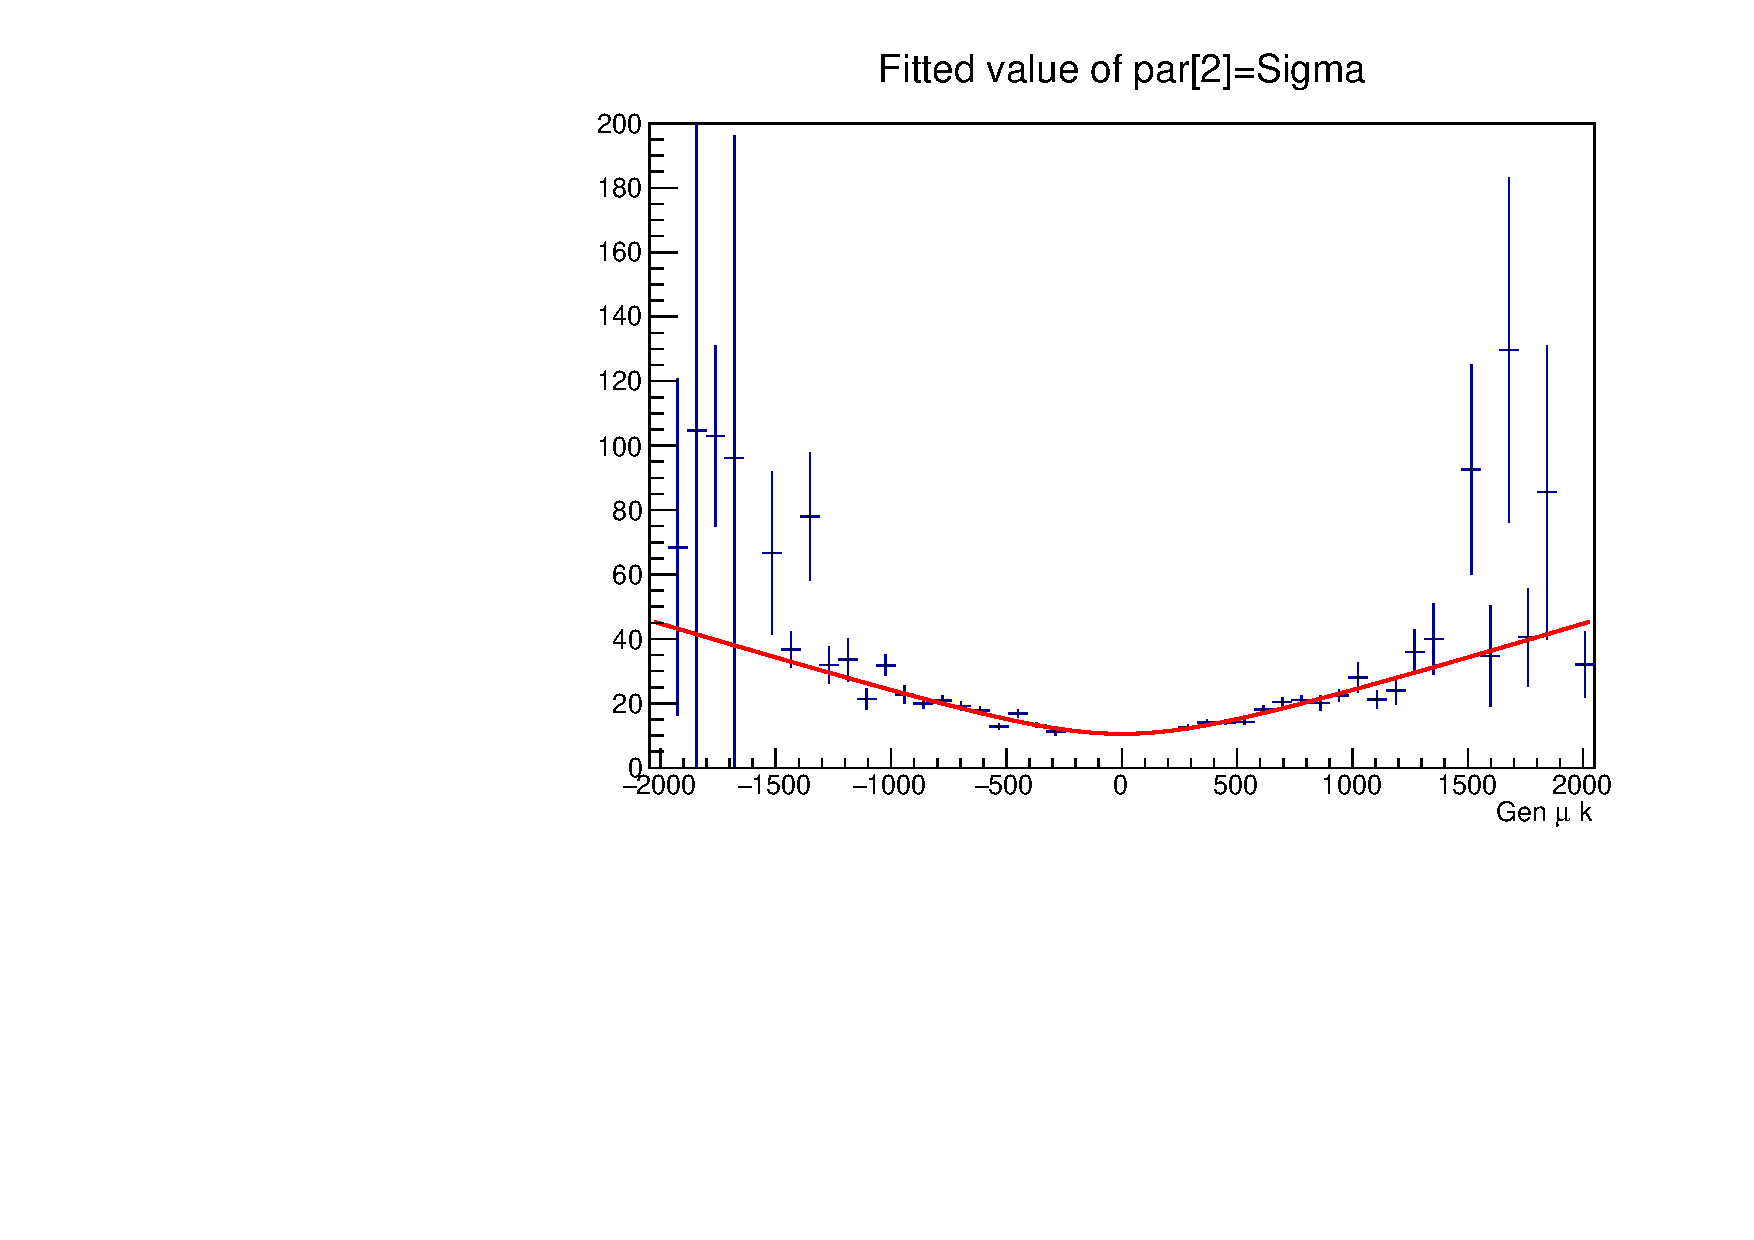
\includegraphics[width=0.45\linewidth]{figs/04_muons/phiprop_sigma.pdf}
	\label{fig:2dprop_sigma}
	\caption[$\sigma$ of vertical slice fits of the 2-dimensional histogram in figure~\ref{fig:2dprop} used to calculate uncertainty coefficients.]
	{$\sigma$ of vertical slice fits of the 2-dimensional histogram in figure~\ref{fig:2dprop} used to calculate uncertainty coefficients.}
	\label{fig:phi_uncertainty}
\end{figure}

Each stub has a measured value representing the "quality" of the hits, with higher values representing a more precise reconstruction of the bending angle. For this reason, the $\phi_b$ position resolutions are calculated separately for high and low quality stubs, as the uncertainty can differ by over a factor of 10 between the two. 

Since the muon detectors only measure $\phi$ and $\phi_b$, the matrix $H$ described in equation~\ref{eq:changeOfBasis} must be a 2$\times$3 matrix that takes the form
\begin{equation}
	H=\left(\begin{matrix}
		0 & 1 & 0\\
		0 & 0 & 1\end{matrix}\right)
\end{equation}

From this, the Kalman Gain $K'$ defined in equation~\ref{eq:gain2} must be a 3x2 matrix with indices $K_{ij}$, and the update step can be explicitly written as
\begin{equation} \label{eq:kmtfUpdate}
	\begin{split}
		k_n^\mathrm{upd}=k_{n-1}+K_{00}\Delta\phi+K_{01}\Delta\phi_b \\
		\phi_n^\mathrm{upd}=\phi_n^\mathrm{prop}+K_{10}\Delta\phi+K_{11}\Delta\phi_b \\
		\phi_{b,n}^\mathrm{upd}=\phi_{b,n}^\mathrm{prop}+K_{20}\Delta\phi+K_{21}\Delta\phi_b
	\end{split}
\end{equation}
where $\Delta\phi$ and $\Delta\phi_b$ are the residuals for $\phi$ and $\phi_b$.

\subsection{Initial Curvature Assignment} \label{sec:kmtf_initk}
The propagation done by the KBMTF presupposes the curvature of the muon is known in order to calculate the $\phi$ and $\phi_b$ at the next station. In order to assign an initial value of the curvature to the track, we use the $\phi_b$ of the seed. Take a muon track beginning at the vertex, and align the axis so the initial bending angle $\phi_{b,0}=0$ as seen in figure~\ref{fig:mu_prop_vertex}. Equation~\ref{eq:parabola2} then becomes
\begin{equation}
	y(x)=akx^2
\end{equation}
From this, we can calculate the $\Delta\phi$ of the muon stub located a distance $R$ from the vertex as
\begin{equation}
	\Delta\phi\approx\frac{y(R)}{R}=akR\\
\end{equation}
The bending angle can then be calculated to be
\begin{equation}
	\phi_b\approx y'(R)-\Delta\phi=akR
\end{equation}

\begin{figure}[htb!]
	\centering
	% !TEX = root../../thesis.tex
\begin{tikzpicture}
	% axis system
	\draw[thick,->] (0,0) -- (10, 0) node[anchor=west] {x};
	\draw[thick,->] (0,-3) -- (0, 3) node[anchor=south] {y};
	\node at (0,0)[circle,fill,inner sep=2pt]{};
	\draw[{Latex[length=3mm]}-,domain=40:0] plot ({15*sin(\x)}, {15-15*cos(\x)});
	\draw ({15*sin(40)}, {15-15*cos(40)}) node[font=\bfseries,anchor=west]{$\mu$};

	\draw[<->] (0, -.5) -- (7, -.5);
	\coordinate[label=below:$R$] (r) at (3.4, -.5);
	\draw[dashed] (7, 0) -- (7, 3);
\end{tikzpicture}
	\caption[Coordinate system for muon propagation beginning at the vertex and going outward.]{Coordinate system for muon propagation beginning at the vertex and going outward.}
	\label{fig:mu_prop_vertex}
\end{figure}
From this, we can see that $\phi_b=\Delta\phi\propto k$. When propagating from the vertex, the muon undergoes small but non-negligable energy loss. Assume the energy loss can be modeled by a constant change in momentum $p\to p-\varepsilon$. Then the curvature $k$ goes as
\begin{equation}
	k=\frac{q}{p}\to\frac{q}{p-\varepsilon}=\frac{q/p}{1-\varepsilon/p}=\frac{k}{1-\varepsilon |k|}
\end{equation}
In a similar process to the propagation coefficient calculation, we use simulated samples to plot $k$ versus $\phi_b$ for each station and fit it to the form
\begin{equation}
	k=\frac{a\phi_b}{1+b|\phi_b|}
\end{equation}
Each station then has coefficients $a$ and $b$ that are used to calculate the initial curvature from $\phi_b$.

Although the KBMTF is intended to be agnostic to the origin of the muon when reconstructing tracks, this derivation was done under the assumption that the muon originated from the vertex. We assign the initial curvature high uncertainty when setting the initial covariance matrix in order to avoid biasing the fit.

\subsection{Quality Cuts on Reconstructed Tracks} \label{sec:kmtf_qual}
The KBMTF requires reconstructed tracks to pass a minimum quality selection in order to reject background. The first measures the goodness of fit of the vertex unconstrained track by propagating the reconstructed track outward and measuring the difference in propagated and measured stub $\phi$ and $\phi_b$. Let the track at the innermost station have curvature, position, and bending angle given by $k$, $\phi^\text{track}$, and $\phi_b^\text{track}$. Applying equations~\ref{eq:prop_phi_approx} and~\ref{eq:prop_phi_approx}  gives
\begin{equation}
	\left(\phi^\text{prop}-\phi^\text{track}\right)+\left(\phi_b^\text{prop}-\phi_b^\text{track}\right)\propto k
\end{equation}
\begin{equation}

\end{equation}

\subsection{Firmware Implementation of the KBMTF} \label{sec:fw}
Two minor approximations are made in order to reduce algorithmic latency and memory usage for firmware implementation. The position resolution of $\phi$ is substantially smaller than the multiple scattering resolution, so the track $\phi$ is set automatically to the measured stub $\phi$. This is equivalent to fixing $K_{10}=1$ and $K_{11}=0$ in equation~\ref{eq:kmtfUpdate}. Secondly, due to the high uncertainty associated with both the measured and propagated $\phi_b$, tracks using three or more stubs set $K_{i1}$ equal to zero and only update using the residual from $\phi$.

Although the Kalman Gain can be exactly calculated exactly given the covariance matrices using equation~\ref{eq:gain}, matrix inversion is a resource and latency expensive process for the hardware based trigger. Implementing division into hardware is significantly more resource intensive than multiplication, so the calculation of the determinant for matrix inversions would cause the algorithm to exceed the latency requirements for real time track finding. Instead, the values of $K_{ij}$ are stored in look-up tables (LUTs) as a function of curvature and the combination of stations that were used to update the track, referred to as the track pattern. For tracks with only two stubs, the LUT contains the exact values of the gain that would have been calculated using equation~\ref{eq:gain2}. For tracks with more than two stubs, this is an approximation that loses some information from updates at previous stations but produces nearly identical performance.

As outlined in section~\ref{sec:kbmtf_cov}, the $\phi_b$ resolution coefficients are different for high and low quality stubs, thus the values for $K_{ij}$ would have to be provided for every possible combination of high and low quality stubs for each track pattern. This would exponentially increase the number of gains stored on LUTs beyond the memory capacity of the hardware. However, from previous approximations, residuals for $\phi_b$ are not used for tracks containing three or more stubs, which fixes $K_{01}$ and $K_{21}$ at 0 for these track patterns. Only gains for track patterns containing two stubs must account for the quality of the stubs. With four stations, this yields six track patterns with four combinations of stub quality that must be stored in LUTs, which is within the capacity of the current hardware.

The firmware is written using Vivado High Level Synthesis (HLS) which compiles firmware written in C to HDL, optimizing it for a given FPGA and clock frequency~\cite{Bachtis:2648953}. When synthesized in a Virtex 7 690T FPGA with a clock frequency of 160\unit{MHz}, the KBMTF algorithm can process a single event in 9 bunch crossings, and is pipelined to allow for continuous processing of events. Table~\ref{tab:kmtfFW} shows the resource utilization of the KBMTF compared to the previous BMTF algorithm, which was implemented using an identical FPGA and clock frequency.

\begin{table} [htb!]
	\centering
	\begin{tabular}{|l|r r r r|}
	\hline
	Algorithm & LUT & FF & BRAM & DSP \\
	\hline
	Phase I BMTF & 43\% & 23\% & 35\% & 0\%\\
	KBMTF & 16\% & 11\% & 15\% & 25\% \\
	\hline 
	\end{tabular}
	\caption[Comparison of FPGA resource utilization~\cite{CERN-LHCC-2020-004}. The KBMTF utilizes DSP cores for arithmetic operations to propagate and update tracks and LUTs for the propagation coefficients and approximate Kalman Gain, while the BMTF uses LUTs to assign momentum.]
	{Comparison of FPGA resource utilization~\cite{CERN-LHCC-2020-004}. The KBMTF utilizes DSP cores for arithmetic operations to propagate and update tracks and LUTs for the propagation coefficients and approximate Kalman Gain, while the BMTF uses LUTs to assign momentum.}
	\label{tab:kmtfFW}
\end{table}

\subsection{Architecture of the KBMTF} \label{sec:kmtf_architecture}
The muon barrel detectors are segmented into 5 wheels along $\hat{z}$, which each wheel composed of 12 sectors in $\phi$ and each sector composed of 4 DT and 3 RPC detectors in $\hat{r}$ as seen in figure~\ref{fig:mu_barrel}. A wedge is defined as the 5 adjacent sectors along all five wheels, shown in figure~\ref{fig:mu_wedge}. 

\begin{figure}[htb!]
	\centering
	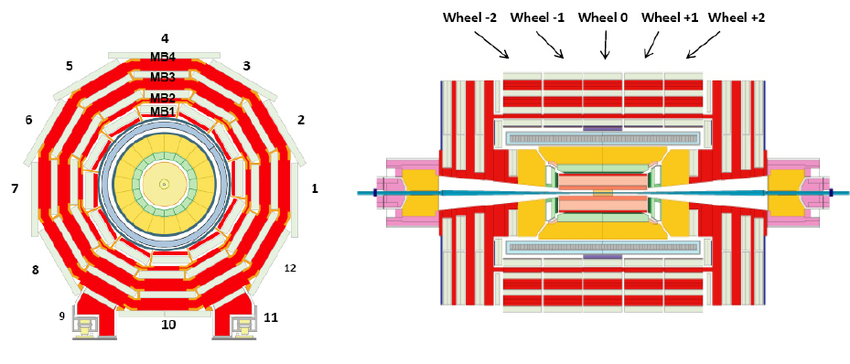
\includegraphics[width=.85\linewidth]{figs/04_muons/muon_barrel.png}
	\caption[Diagram of the CMS muon barrel system~\cite{Chatrchyan_2010}. (Left) Each wheel is segmented in 12 sectors in $\phi$ and 4 DT and 3 RPC stations in $r$. (Right) The 5 wheels in $z$.]{Diagram of the CMS muon barrel system~\cite{Chatrchyan_2010}. (Left) Each wheel is segmented in 12 sectors in $\phi$ and 4 DT and 3 RPC stations in $r$. (Right) The 5 wheels in $z$.}
	\label{fig:mu_barrel}
\end{figure}

The hardware for the KBMTF consists of 12 Master Processor --- Virtex-7 (MP7) boards, each hosting a Xilinx FPGA Virtex-7 chip, which are distributed among two $\mu$TCA crates~\cite{bmtf_hardware}. The FPGA is responsible for receiving inputs from the TwinMux system through high speed optical links, reconstructing muon tracks, and delivering the muon candidates to the global muon trigger. Each MP7 corresponds to a central wedge and receives TwinMux stubs from all stations in both the central wedge and the two adjacent wedges. For a given MP7, the KBMTF algorithm reconstructs all tracks that have an outermost stub in the central wedge before overlap cleaning tracks that share stubs. It then picks the three best muon tracks based on track fit quality and \pt to deliver to the global muon trigger.

\begin{figure}[htb!]
	\centering
	% !TEX = root = ../../thesis.tex
\usetikzlibrary{shapes.geometric}
\usetikzlibrary{calc}
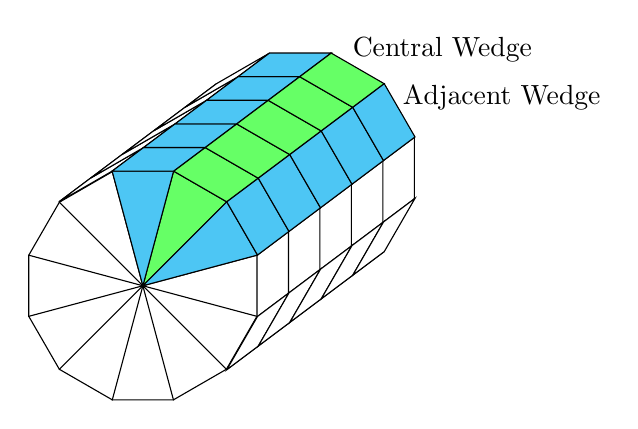
\begin{tikzpicture}

\def\dx{.4};
\def\dy{.3}
\def\r{3}
\def\c{1}
	
\node[draw, fill=white, regular polygon, regular polygon sides=12, minimum size=\r*\c cm] (w6) at (\dx*\c*5,\dy*\c*5){};
	
\node[draw, fill=white, regular polygon, regular polygon sides=12, minimum size=\r*\c cm] (w5) at (\dx*\c*4,\dy*\c*4){};

\node[draw, fill=white, regular polygon, regular polygon sides=12, minimum size=\r*\c cm] (w4) at (\dx*\c*3,\dy*\c*3){};

\node[draw, fill=white, regular polygon, regular polygon sides=12, minimum size=\r*\c cm] (w3) at (\dx*\c*2,\dy*\c*2){};

\node[draw, fill=white, regular polygon, regular polygon sides=12, minimum size=\r*\c cm] (w2) at (\dx*\c*1,\dy*\c*1){};

\node[draw, fill=white, regular polygon, regular polygon sides=12, minimum size=\r*\c cm] (w1) at (0,0){};

\foreach \i in {1,2,3,4,5,6,7,8,9,10,11,12}{
	\draw (0,0) -- (w1.corner \i);
}
\foreach \i in {1,2,3,9,10,11,12}{
	\draw (w1.corner \i) -- (w6.corner \i);
}


% Fixing perspective
\draw[fill=white] (w1.corner 9) -- (w2.corner 9) -- (w2.corner 10) -- (w1.corner 10) -- cycle;
\draw[fill=white] (w2.corner 9) -- (w3.corner 9) -- (w3.corner 10) -- (w2.corner 10) -- cycle;
\draw[fill=white] (w3.corner 9) -- (w4.corner 9) -- (w4.corner 10) -- (w3.corner 10) -- cycle;
\draw[fill=white] (w4.corner 9) -- (w5.corner 9) -- (w5.corner 10) -- (w4.corner 10) -- cycle;
\draw[fill=white] (w5.corner 9) -- (w6.corner 9) -- (w6.corner 10) -- (w5.corner 10) -- cycle;

\draw[fill=white] (w1.corner 2) -- (w2.corner 2) -- (w2.corner 3) -- (w1.corner 3) -- cycle;
\draw[fill=white] (w2.corner 2) -- (w3.corner 2) -- (w3.corner 3) -- (w2.corner 3) -- cycle;
\draw[fill=white] (w3.corner 2) -- (w4.corner 2) -- (w4.corner 3) -- (w3.corner 3) -- cycle;
\draw[fill=white] (w4.corner 2) -- (w5.corner 2) -- (w5.corner 3) -- (w4.corner 3) -- cycle;
\draw[fill=white] (w5.corner 2) -- (w6.corner 2) -- (w6.corner 3) -- (w5.corner 3) -- cycle;

% Central wedge
\draw[fill=green!60] (w1.corner 12) -- (w1.corner 1) -- (0,0) -- cycle;
\draw[fill=green!60] (w1.corner 12) -- (w2.corner 12) -- (w2.corner 1) -- (w1.corner 1) -- cycle;
\draw[fill=green!60] (w2.corner 12) -- (w3.corner 12) -- (w3.corner 1) -- (w2.corner 1) -- cycle;
\draw[fill=green!60] (w3.corner 12) -- (w4.corner 12) -- (w4.corner 1) -- (w3.corner 1) -- cycle;
\draw[fill=green!60] (w4.corner 12) -- (w5.corner 12) -- (w5.corner 1) -- (w4.corner 1) -- cycle;
\draw[fill=green!60] (w5.corner 12) -- (w6.corner 12) -- (w6.corner 1) -- (w5.corner 1) -- cycle;

% Adjacent wedge +1
\draw[fill=cyan!70] (w1.corner 11) -- (w1.corner 12) -- (0,0) -- cycle;
\draw[fill=cyan!70] (w1.corner 12) -- (w2.corner 12) -- (w2.corner 11) -- (w1.corner 11) -- cycle;
\draw[fill=cyan!70] (w2.corner 12) -- (w3.corner 12) -- (w3.corner 11) -- (w2.corner 11) -- cycle;
\draw[fill=cyan!70] (w3.corner 12) -- (w4.corner 12) -- (w4.corner 11) -- (w3.corner 11) -- cycle;
\draw[fill=cyan!70] (w4.corner 12) -- (w5.corner 12) -- (w5.corner 11) -- (w4.corner 11) -- cycle;
\draw[fill=cyan!70] (w5.corner 12) -- (w6.corner 12) -- (w6.corner 11) -- (w5.corner 11) -- cycle;
% Adjacent wedge -1

\draw[fill=cyan!70] (w1.corner 1) -- (w1.corner 2) -- (0,0) -- cycle;
\draw[fill=cyan!70] (w1.corner 2) -- (w2.corner 2) -- (w2.corner 1) -- (w1.corner 1) -- cycle;
\draw[fill=cyan!70] (w2.corner 2) -- (w3.corner 2) -- (w3.corner 1) -- (w2.corner 1) -- cycle;
\draw[fill=cyan!70] (w3.corner 2) -- (w4.corner 2) -- (w4.corner 1) -- (w3.corner 1) -- cycle;
\draw[fill=cyan!70] (w4.corner 2) -- (w5.corner 2) -- (w5.corner 1) -- (w4.corner 1) -- cycle;
\draw[fill=cyan!70] (w5.corner 2) -- (w6.corner 2) -- (w6.corner 1) -- (w5.corner 1) -- cycle;

%\node[text=green!60, label={right:Central Wedge}] at ($(w6.corner 12)!0.5!(w6.corner 1)$){};
\node[label={[right]:Central Wedge}, xshift=1ex, yshift=-.5ex] at (w6.corner 1){};
\node[label={[right]:Adjacent Wedge},xshift=0.75ex, yshift=-2ex] at (w6.corner 12){};

\end{tikzpicture}

	\caption[Diagram showing the inputs of one MP7 board consisting, consisting of the TwinMux inputs from one central wedge (green) and the two adjacent wedges (blue). The FPGA reconstructs all tracks with the outermost stub in the central wedge.]{Diagram showing the inputs of one MP7 board consisting, consisting of the TwinMux inputs from one central wedge (green) and the two adjacent wedges (blue). The FPGA reconstructs all tracks with the outermost stub in the central wedge.}
	\label{fig:mu_wedge}
\end{figure}

\section{Performance of the Kalman Barrel Muon Track Finder} \label{sec:kmtf_performance}
The performance of an trigger algorithm is primarily determined by the rate and efficiency. The efficiency is the fraction of signal events that successfully have a track reconstructed by the algorithm, while the rate is the frequency that the algorithm will trigger. A high efficiency is desirable to ensure any interesting events are stored for future analysis, while a low rate is crucial to reject background events and provide a reasonable bandwidth to store events.

\subsection{Trigger Efficiencies and Rate} \label{sec:kmtf_eff}
The previous L1 barrel muon trigger (BMTF) functioned by using pairs of stubs to form tracks, then using a LUT to assign track parameters based on the $\phi$ and $\phi_b$ of the stubs. This LUT takes only the $\phi$ and $\phi_b$ of the two stubs and was calculated with the assumption that the muon originated from the beam axis. In the case of displaced muons, which arise from secondary decays of long lived, beyond standard model particles, the assumption is no longer valid and results in large inefficiencies as the muon becomes more displaced from the beam axis.

The general efficiency of a trigger is defined as the fraction of signal muons that have a matching reconstructed track, and can be expressed abstractly as

\begin{equation}\label{eq:eff}
	\epsilon=\frac{N_\mathrm{signal}(\mathrm{Passing\ trigger})}{N_\mathrm{signal}}	
\end{equation}

For muon triggers, the denominator of signal muons consist of events that have known information about the muons. This can be from generator information in simulated monte-carlo samples, tracker information using cosmic muon data, or probe muons using the tag-and-probe method on data. These signal muons are cut using the known muon information to produce a reasonable sample for track reconstruction. The numerator consists of signal muons with a matching reconstructed track that may have addition cuts on the reconstructed track properties.

Figure~\ref{fig:eff_KmtfVsBmtf} shows the efficiencies calculated on probe muons from a Z boson tag-and-probe sample collected during 2017 data taking. The associated tracker tracks for the probe muons are used as the known information, while the associated stubs are used to run the L1 muon reconstruction algorithms. Figure~\ref{fig:effVsPt} shows the efficiency versus track \pt comparing the KBMTF and phase-1 BMTF algorithm, with the requirement that the matching L1 tracks have $\pt>20\GeV$. This requirement creates the turn-on curve effect, which has a sharpness proportional to the muon momentum resolution, followed by the plateau at which the algorithms reach maximum efficiency. Figure~\ref{fig:effVsEta} shows the same efficiencies versus track $\eta$, with the additional requirement that the tracker tracks have $\pt>25\GeV$ in order to show the efficiency on the plateau. Quality cuts in the KBMTF algorithm were tuned to match the efficiency of the BMTF.

\begin{figure}[htb!]
	\centering
	\captionsetup[subfigure]{justification=centering}
	\begin{subfigure}[h]{0.45\linewidth}
		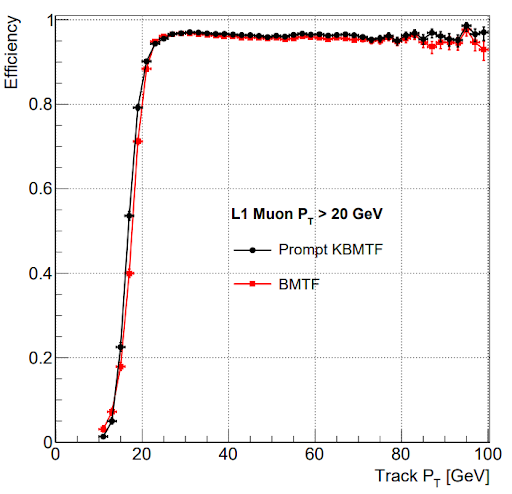
\includegraphics[width=\linewidth]{figs/04_muons/effVsPt_kmtf.png}
		\caption{Efficiency versus track \pt}
		\label{fig:effVsPt}
	\end{subfigure}
	\begin{subfigure}[h]{0.45\linewidth}
		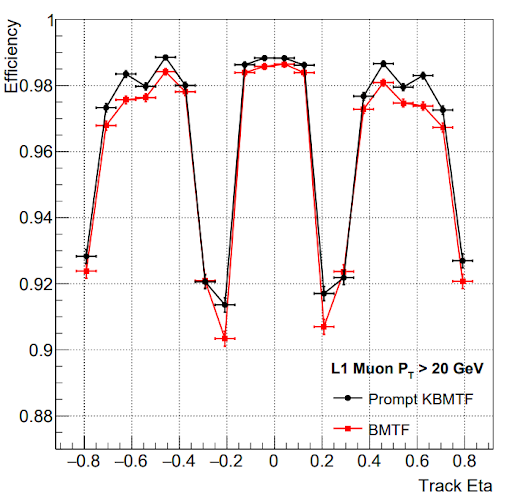
\includegraphics[width=\linewidth]{figs/04_muons/effVsEta_kmtf.png}
		\caption{Efficiency versus track $\eta$}
		\label{fig:effVsEta}
	\end{subfigure}
	\caption[Comparison of efficiencies between the KBMTF and phase-1 BMTF algorithm using a Z tag-and-probe sample collected during 2017 data taking. (a) Efficiency versus track \pt, requiring L1 muon $\pt>20\GeV$. (b) Efficiency versus track $\eta$, requiring L1 muon $\pt>20\GeV$ and track $\pt>25\GeV$ in order to show the efficiency on the plateau. The drops in efficiency at $\eta=\pm0.2$ are due to gaps between wheels in the muon system.]{Comparison of efficiencies between the KBMTF and phase-1 BMTF algorithm using a Z tag-and-probe sample collected during 2017 data taking. (a) Efficiency versus track \pt, requiring L1 muon $\pt>20\GeV$. (b) Efficiency versus track $\eta$, requiring level-1 muon $\pt>20\GeV$ and track $\pt>25\GeV$ in order to show the efficiency on the plateau. The drops in efficiency at $\eta=\pm0.2$ are due to gaps between wheels in the muon system.}
	\label{fig:eff_KmtfVsBmtf}
\end{figure}

Figure~\ref{fig:effVsDxy_kmtf} shows the efficiency versus muon $d_{xy}$ for three track finding algorithms. The denominator consists of cosmic ray muons passing through the barrel muon detectors with a $p_T>20\GeV$. The numerator requires a matching L1 track with reconstructed $p_T>10\GeV$. The lower threshold for the L1 track is set to prevent the momentum resolution of the reconstruction algorithms from affecting the efficiency. The first algorithm is the BMTF, which shows inefficiencies due to the $p_T$ LUTs assuming the muon originated at the beam axis. The second is the prompt KBMTF, which uses the vertex constrained measurement. This also shows inefficiencies due to the vertex constraint, but is better than the BMTF as the vertex constraint isn't applied until the last step of track reconstruction. Lastly, the displaced KBMTF uses the vertex unconstrained measurement and shows substantial improvements compared to both prompt algorithms.

\begin{figure}[htbp!]
	\centering
	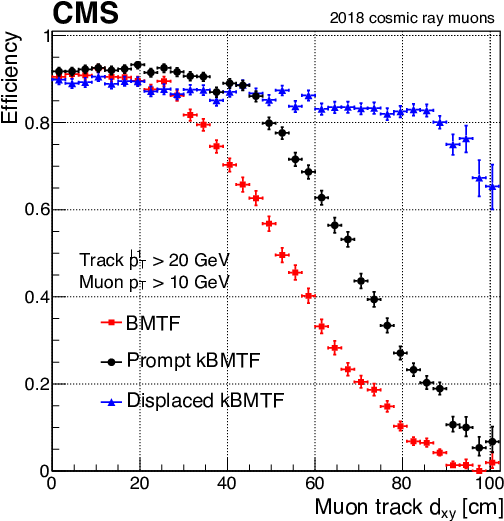
\includegraphics[width=0.5\linewidth]{figs/04_muons/effVsDxy_kmtf.png}
	\caption[Comparison of efficiency vs cosmic track $d_{xy}$ using cosmic data from the 2018 data taking run. The prompt KBMTF takes the reconstructed $p_{T}$ using the vertex constrained measurement, while the displaced KBMTF uses the vertex unconstrained measurement. The displaced KBMTF shows substantial improvements to the previous BMTF~\cite{Hayrapetyan:2870088}]
	{Comparison of efficiency vs cosmic track $d_{xy}$ using cosmic data from the 2018 data taking run. The prompt KBMTF takes the reconstructed $p_{T}$ using the vertex constrained measurement, while the displaced KBMTF uses the vertex unconstrained measurement. The displaced KBMTF shows substantial improvements to the previous BMTF~\cite{Hayrapetyan:2870088}.}
	\label{fig:effVsDxy_kmtf}
\end{figure}

A reconstructed track must have a $p_T$ above a given threshold to trigger on an event. Thresholds are set to optimize the analysis potential of the data while also minimizing the additional bandwidth to store events. The rate, which is the frequency at which a trigger decides to store an event, can be calculated as a function of threshold using zero bias data, which is collected by storing random events regardless of trigger acceptance. This creates a representative data set of all $pp$ collisions, hence the name "zero bias". The rate can be calculated from the zero bias data as follows
\begin{equation}
	\mathrm{R} = f_\mathrm{rev}\times \left<N_\mathrm{bunches}\right>\times\frac{N_\mathrm{events}(\mathrm{L1}\ \mathrm{Track}\ p_{T}>\mathrm{Threshold})}{N_\mathrm{events}}
\end{equation}
Where $f_\mathrm{rev}$ is the LHC revolution frequency of 11.245\unit{kHz} and $\left<N_\mathrm{bunches}\right>$ is the average number of proton bunches that will collide in one revolution. For 2017 data taking these yield a scale factor of 20984$\unit{kHz}$. Figure~\ref{fig:kmtf_rate} shows the rate versus threshold for the BMTF, vertex constrained KBMTF, and vertex unconstrained KBMTF. The KBMTF was tuned for similar efficiency but lower rate than the BMTF at 20\GeV. The displaced KBMTF initially shows lower rate at low \pt thresholds due to scale corrections to the reconstructed muon momentum.

\begin{figure}[htbp!]
	\centering
	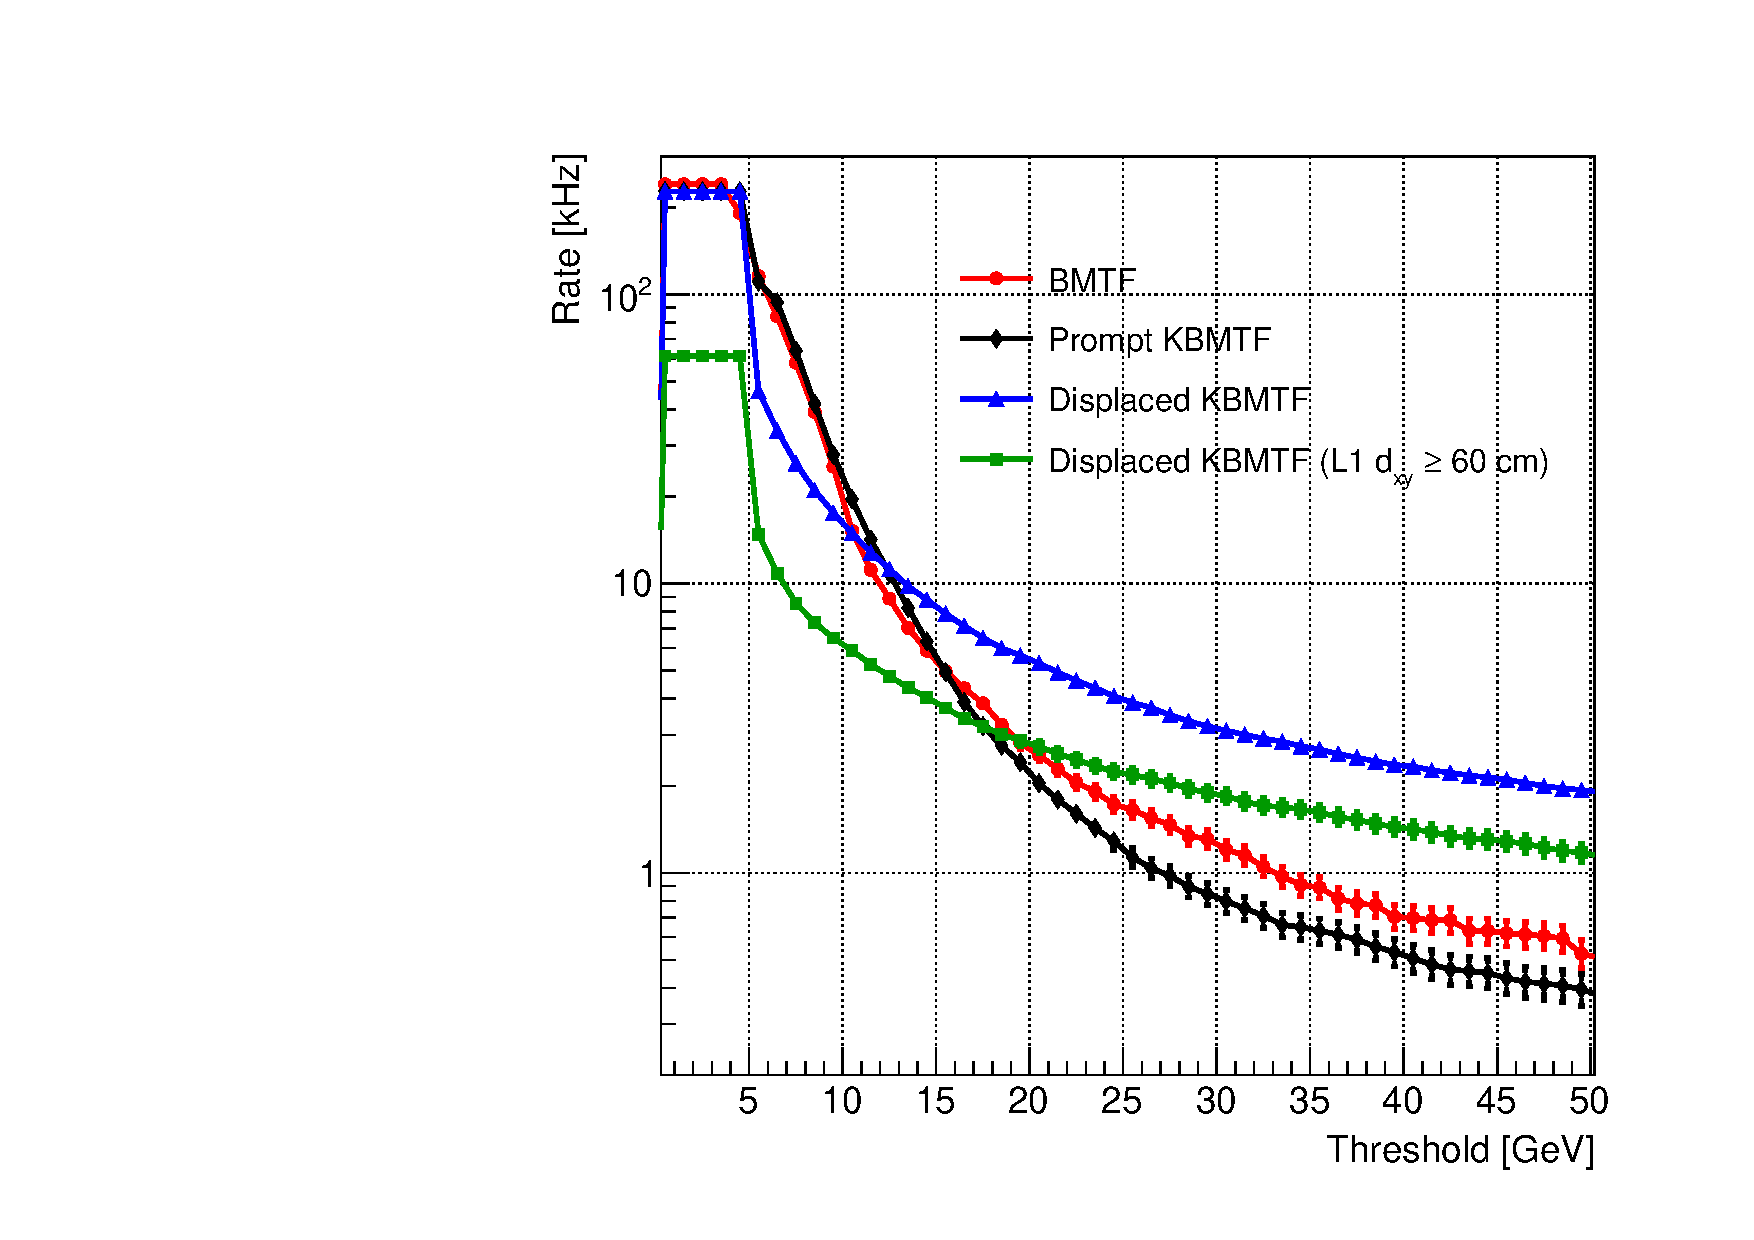
\includegraphics[width=0.5\linewidth]{figs/04_muons/rate_kmtf.pdf}
	\caption[Rate comparison calculated using 2017 zero bias data of the Phase I BMTF, vertex constrained (prompt) KBMTF, vertex unconstrained (displaced) KBMTF, and displaced KBMTF for displaced tracks.]{Rate comparison calculated using 2017 zero bias data of the Phase I BMTF, vertex constrained (prompt) KBMTF, vertex unconstrained (displaced) KBMTF, and displaced KBMTF for displaced tracks.}
	\label{fig:kmtf_rate}
\end{figure}

\subsection{Firmware and Emulator Agreement} \label{sec:kmtf_fwVsEmu}
The performance of the KBMTF is tested using a dedicated C++ software emulator which is integrated into the CMS analysis framework. This emulator follows similar logic to the HLS code, but is not a one-to-one replica. Several modifications are made to the HLS code in order to make it compatible with the synthesis into HDL and pipelining. As such, a test bench is used to ensure that the output of the firmware and emulator are identical. The emulator runs the algorithm over several events and outputs a text file containing information on the input stubs and the reconstructed tracks. This text file is used as input for the test bench, which runs the stub information through the HLS code and compares the properties of the reconstructed tracks to those found in the emulator.

Disagreements between the emulator and firmware are used for a variety of debugging purposes. They frequently point to logic errors in the simplification of the algorithm for HLS synthesis, or in other cases show flaws in the emulator. During Run 2, the disagreements were almost entirely due to differences resulting from fixed point calculations in the firmware compared to floating point calculations in the emulator. These differences have been drastically reduced due to the addition of C++ classes that mimic fixed point calculations in the emulator, which now has a $>$99.9\% agreement to the firmware. Figure~\ref{fig:kmtf_rate} shows a comparison of the outputs of the firmware and emulator using events from a 2017 Z tag-and-probe sample.

\begin{figure}[htb!]
	\centering
	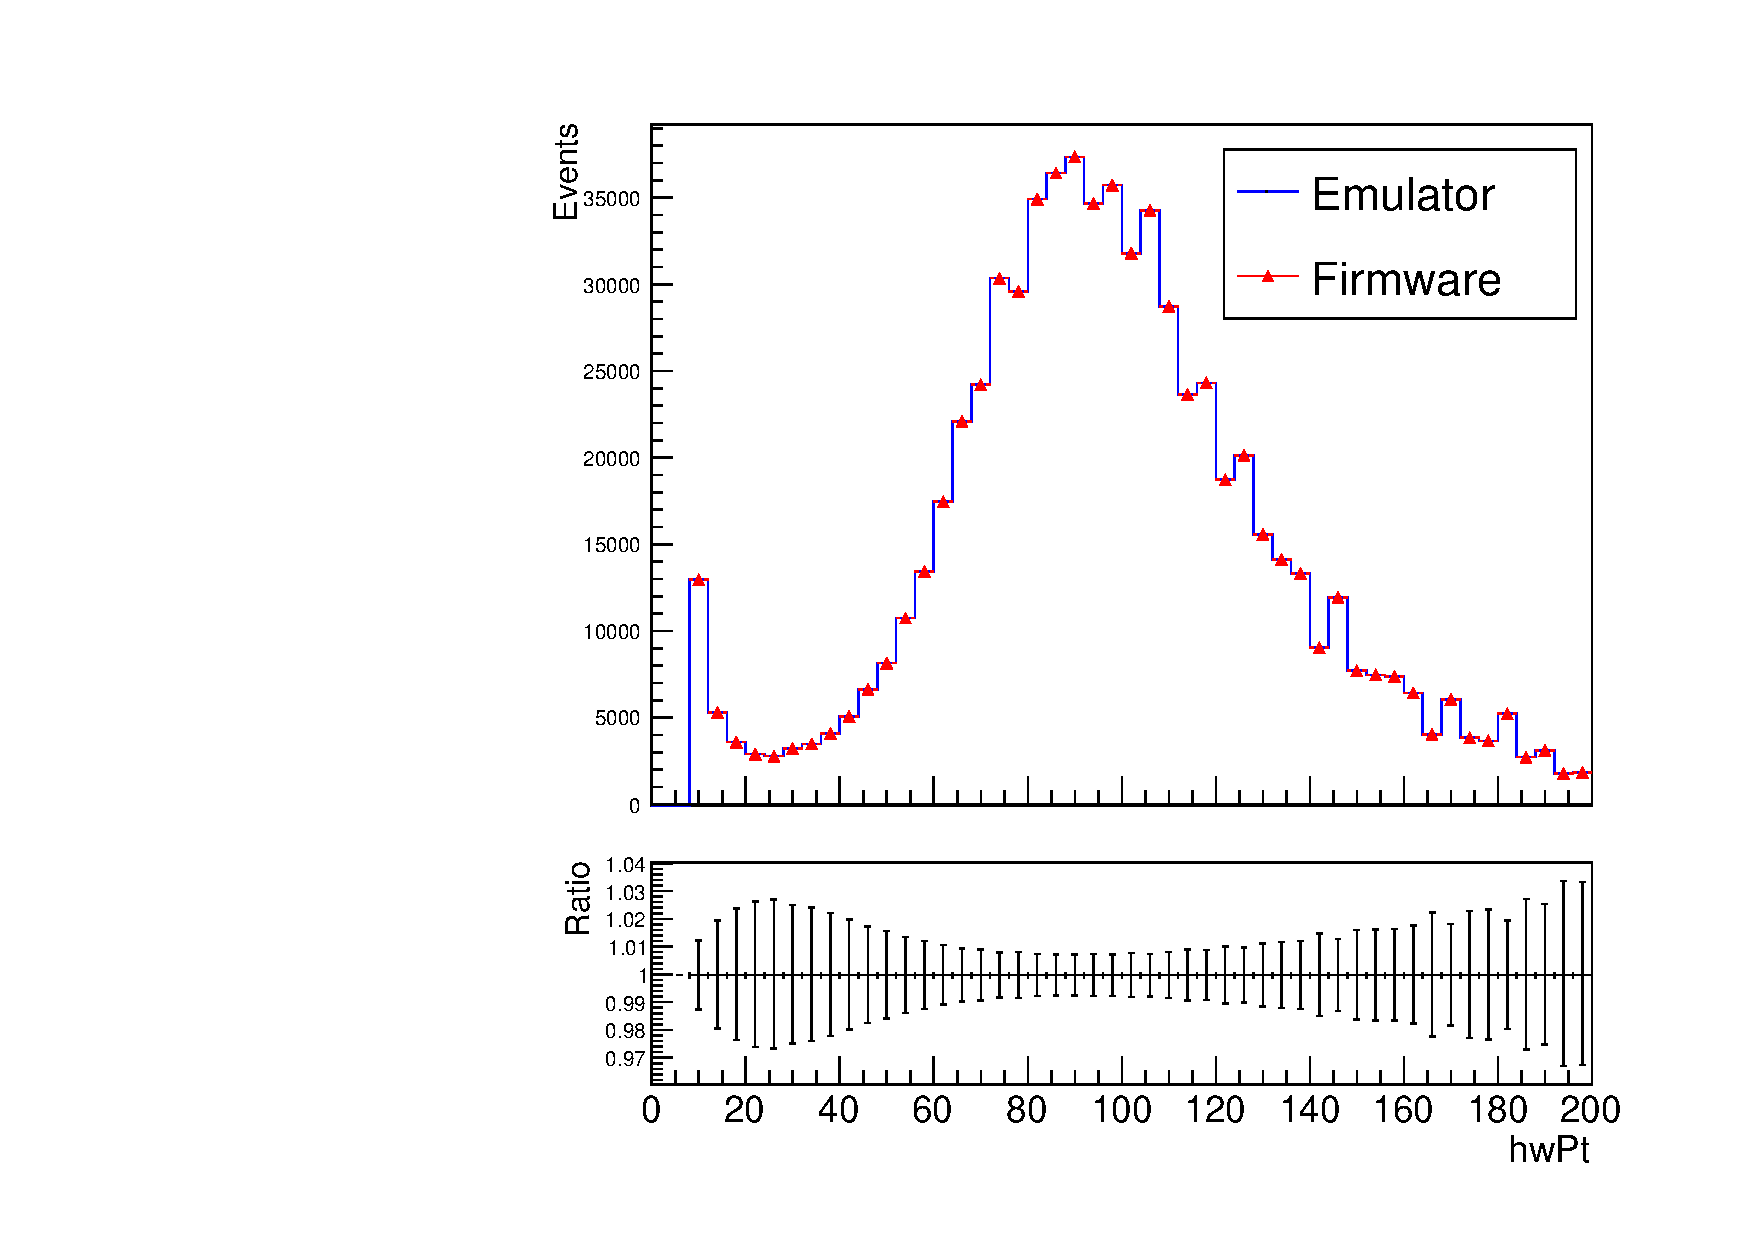
\includegraphics[width=0.55\linewidth]{figs/04_muons/emuVsFw_pt.pdf}
	\caption[Comparison of the track $p_T$ between the firmware and emulator using data from a 2017 Z tag-and-probe sample. hwPt represents the integer value of p$_T$ used in hardware. The emulator and firmware output show 100\% agreement across 500000 events.]{Comparison of the track $p_T$ between the firmware and emulator using data from a 2017 Z tag-and-probe sample. hwPt represents the integer value of p$_T$ used in hardware. The emulator and firmware output show 100\% agreement across 500000 events.}
	\label{fig:kmtf_fwVsEmu}
\end{figure}

\section{The Phase-2 KBMTF} \label{sec:HL_KBMTF}
The modifications to the KBMTF algorithm for the HL-LHC result from increased precision from the input trigger primitives and modifications to the trigger architecture. These changes mainly affect the firmware implementation and do not require conceptual changes to the logic used to propagate and update tracks. The propagation coefficients and Kalman Gain must be recalculated as the number of bits allocated to $k$, $\phi$, and $\phi_b$ change. Additionally, the firmware will receive primitives from the entire barrel muon system simultaneously as opposed to processing each sector in $\phi$ independently. The firmware will be time-multiplexed with a factor of 18, meaning data from each event will be sent to one of 18 processors running the KBMTF algorithm in parallel. Additionally, the FPGA will be changed to a ZYNQ Ultrascale+ and synthesized at a clock frequency of 200\unit{MHz}. Simulations show a resource utilization of 17\% LUT, 3\% FF, 11\% DSP, and 7\% BRAM~\cite{CERN-LHCC-2020-004}.

The KBMTF algorithm performance is robust to the high pileup conditions of the HL-LHC. The efficiencies remain the same as Phase-1, and the rate scales approximately linearly with pileup as expected. Figure~\ref{fig:rate_eff_HLLHC} shows the efficiency versus generated muon $p_T$, single muon rates versus threshold, and single muon rates versus pileup for the Phase-2 KBMTF and two proposed track finding algorithms. As discussed in section~\ref{sec:CMS_L1T}, the HL-LHC track trigger introduces new track primitives that will be used in novel muon triggers. These new algorithms have higher efficiency and precision for prompt muons due to the momentum resolution of the tracker, but will be unable to trigger on displaced muons as the track primitives do not include displaced tracks. 

\begin{figure} [htb!]
	\centering
	\captionsetup[subfigure]{justification=centering}
	\begin{subfigure}[h]{0.45\linewidth}
		\centering
		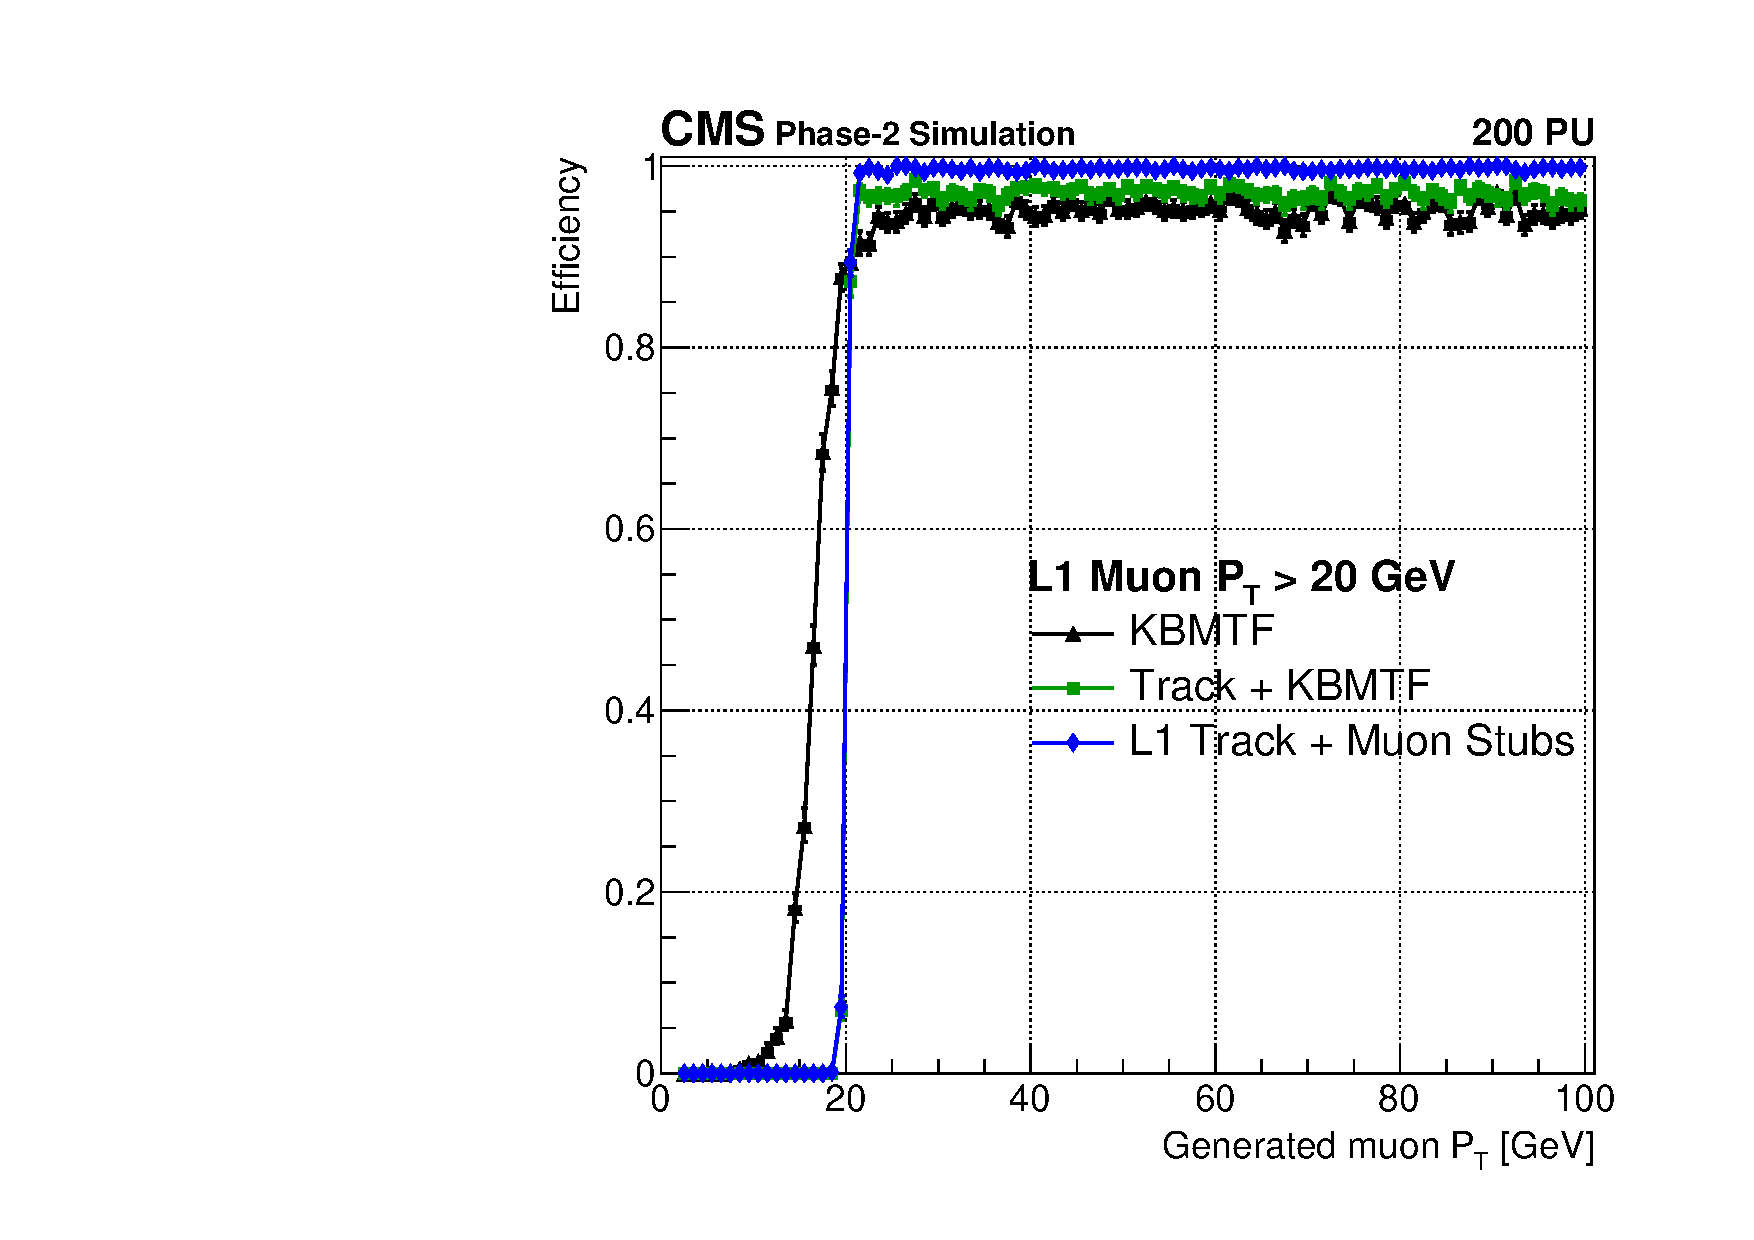
\includegraphics[width=\linewidth]{figs/04_muons/effVsPt_20_TPS.pdf}
		\caption{Efficiency vs gen $\mu$ $p_T$.}
		\label{}
	\end{subfigure} \hspace{0.05\linewidth}
	\begin{subfigure}[h]{0.45\linewidth}
		\centering
		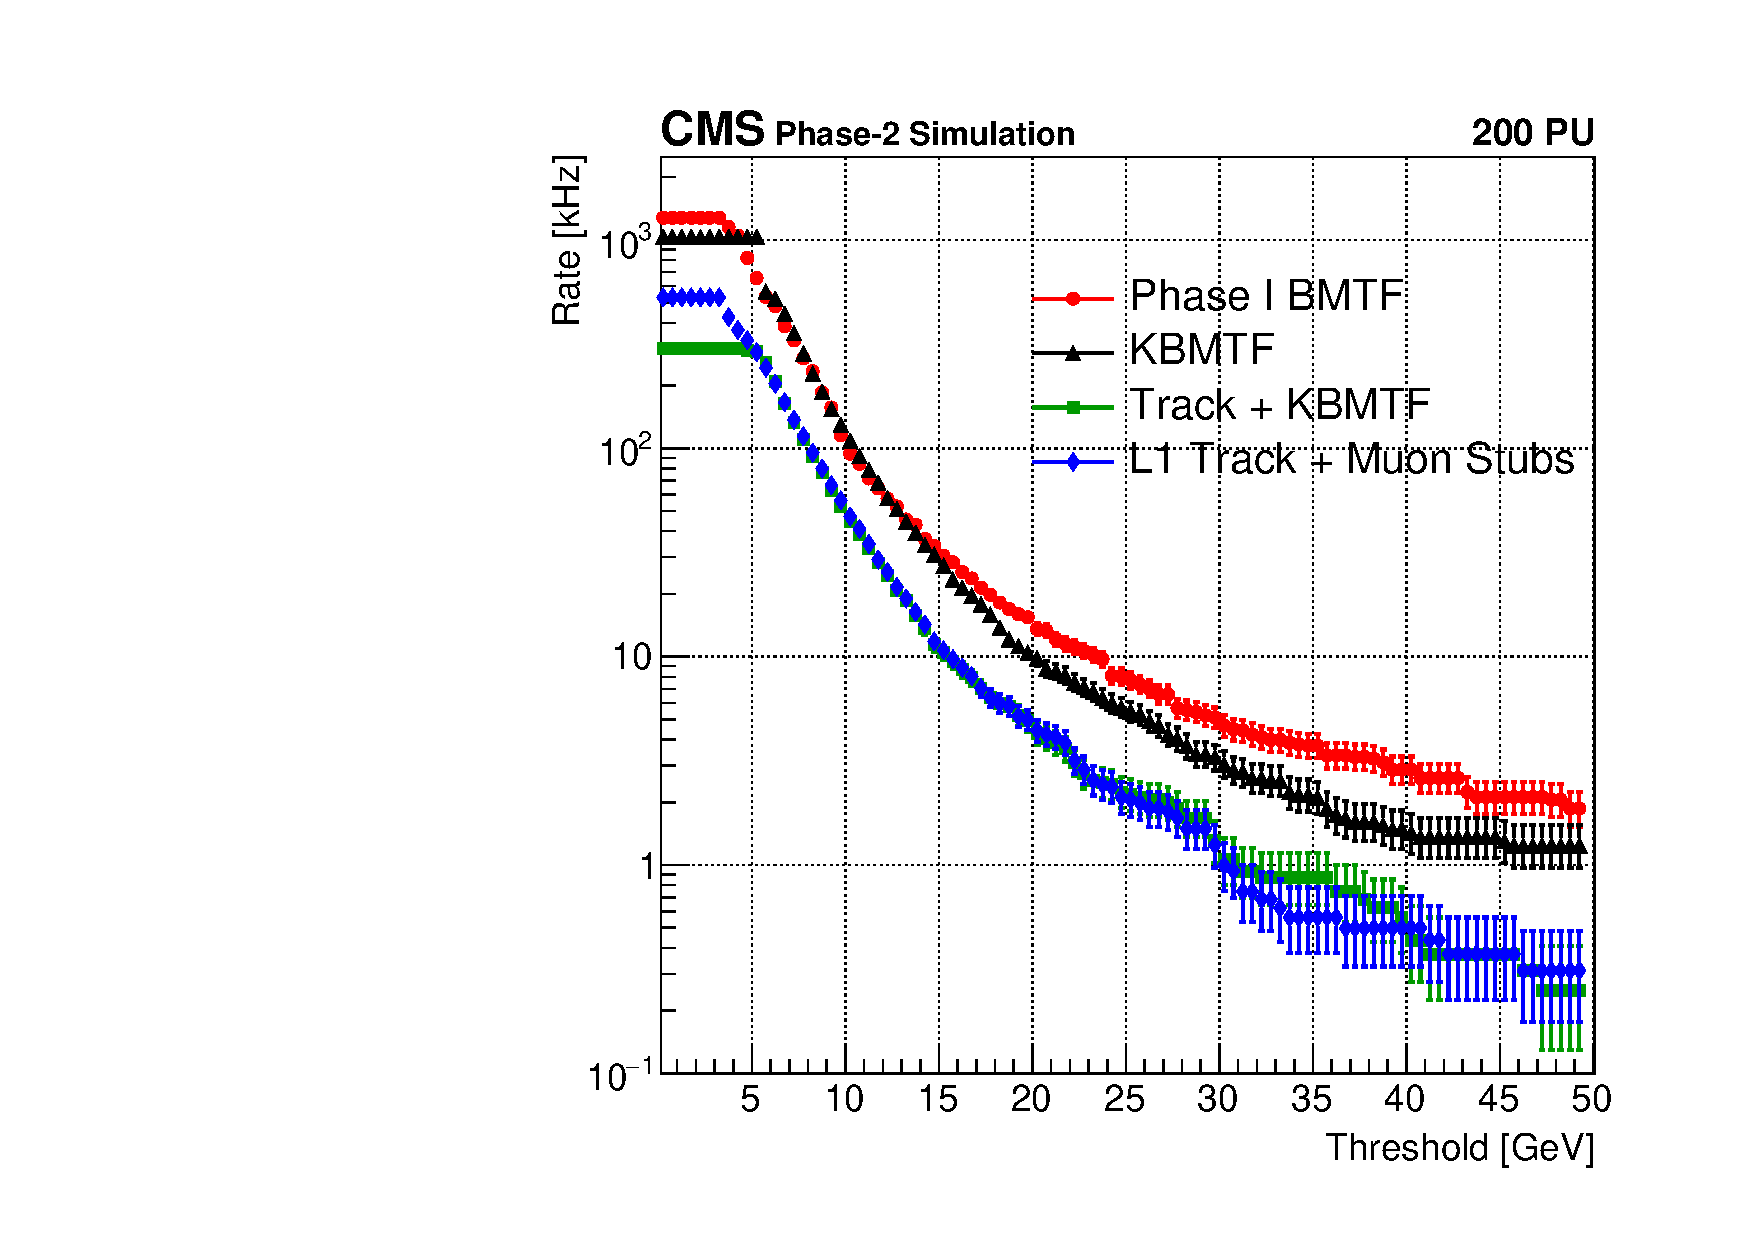
\includegraphics[width=\linewidth]{figs/04_muons/rateVsPt_TPS.pdf}
		\caption{Single muon rates versus threshold.}
		\label{}
	\end{subfigure}
	\begin{subfigure}[h]{0.45\linewidth}
		\centering
		\includegraphics[width=\linewidth]{figs/04_muons/rateVsPU_TPS.pdf}
		\caption{Single muon rates vs pileup for a 20\GeV threshold~\cite{CERN-LHCC-2020-004}}
		\label{}
	\end{subfigure}
	\caption[Performance of the L1 Barrel Muon algorithms using simulated samples with HL-LHC run conditions. The Track + KBMTF algorithm matches tracks to loose KBMTF muons, while the L1 Track + Muon Stubs algorithm matches tracks to muon stubs.]{Performance of the L1 Barrel Muon algorithms using simulated samples with HL-LHC run conditions. The Track + KBMTF algorithm matches tracks to loose KBMTF muons, while the L1 Track + Muon Stubs algorithm matches tracks to muon stubs.}
	\label{fig:rate_eff_HLLHC}
\end{figure}